%!TeX TS-program = pdflatex
%!TeX encoding = UTF-8 Unicode
%!TeX spellcheck = en-US
%!BIB TS-program = bibtex
% -*- coding: UTF-8; -*-
% vim: set fenc=utf-8

%%%%%%%%%%%%%%%%%%%%%%%%%%%%%%%%%%%%%%%%%%%%%%%%%%%%%%%%%%%%%%%%%%%%%
\newcommand{\AuthorA}{Chlo\'e Pasturel}
\newcommand{\AuthorB}{Anna Montagnini}%
\newcommand{\AuthorC}{Laurent U.~Perrinet}%

\newcommand{\Address}{Institut de Neurosciences de la Timone, CNRS / Aix-Marseille Universit\'e - Marseille, France}%

%\newcommand{\Website}{http://invibe.net/LaurentPerrinet}%
%\newcommand{\Email}{Laurent.Perrinet@univ-amu.fr}%

\newcommand{\Title}{ANEMO : Quantitative tools for the ANalysis of Eye MOvements}
%\newcommand{\Conference}{GDR Vision 2017 / Lille, France \\
%Acknowledgments : ANR grant <<Reinforcement and Eye Movements>> \textbf{ANR-13-APPR-0008-02}}%

\newcommand{\Conference}{\textbf{	
Grenoble Workshop on Models and Analysis of Eye Movements}, Grenoble, France - code and material @ \url{https://github.com/invibe/ANEMO} \\\\\\\\\\\\\\\\\\\\\\\\\\\\\\\\\\\\\\\\\\\\\\\\\\\\\\\\\\\\\\\\\\\\\\\\\\\\\\\\\\\\\\\\\\\\\\\\ Acknowledgments : EU Horizon 2020 ITN MSC grant <<PACE>> n.642961}
%%%%%%%%%%%%%%%%%%%%%%%%%%%%%%%%%%%%%%%%%%
\documentclass[profile,final,english, draft]{sciposter}%landscape,french]{sciposter}% ,draft]{sciposter}% 
\usepackage{babel}
% MATHS (AMS)
\usepackage{amsmath}
\usepackage{amsfonts} 
\usepackage{amssymb}
\usepackage{amsthm}
\newtheorem*{thm}{Proposition}


%% ========  polices de caracteres =============
\usepackage[T1]{fontenc}% 
\usepackage{lmodern}%
\usepackage{t1enc}
\usepackage{ragged2e}
%============ graphics ===================
\usepackage[pdftex]{graphicx}% 
\DeclareGraphicsExtensions{.pdf,.png, .jpg}%
\graphicspath{{./figures/}}%
%\usepackage[numbers,comma,sort&compress,round]{natbib} %
\usepackage[%style=nature,
maxcitenames=2,
maxnames = 2,
firstinits=true,
uniquename=init,
sorting=none,
url=false,
isbn=false,
eprint=false,
texencoding=latin1,
bibencoding=utf8,
autocite=superscript,
backend=bibtex,
%articletitle=false
]{biblatex}%

\addbibresource{Pasturel_etal2017gdr.bib}%
%%%%%%%%%%%%%%%%%%%%%%%%%%%%%%
%% OPTIONAL MACRO FILES
%\usepackage{tikz,tkz-euclide} \usetkzobj{all} % loading all objects
%\usetikzlibrary{positioning} \usetikzlibrary{calc}
%\usepackage{sfmath}
%============ hyperref ===================
\usepackage[unicode,linkcolor=red,citecolor=red,filecolor=black,urlcolor=red,pdfborder={0 0 0}]{hyperref}%
\hypersetup{%
pdftitle={\Title},%
pdfauthor={\AuthorA},%< \Email > \Address},%
pdfsubject={\Conference}%
}%
\usepackage{color,multicol}%
%%============= margins ==================
\setlength{\columnseprule}{.05mm}
\makeatletter
\renewcommand{\section}{\@startsection
        {section}%              % the name 
        {1}%                    % the level
        {0mm}%                  % the indent
        {0\baselineskip}%      % the beforeskip
        {0.2\baselineskip}%                  % the afterskip
        {\LARGE\color{red}\bfseries}}% % the style
\renewcommand{\subsection}{\@startsection
        {subsection}%              % the name 
        {2}%                    % the level
        {0mm}%                  % the indent
        {0\baselineskip}%      % the beforeskip
        {0.1\baselineskip}%                  % the afterskip
        {\Large\color[rgb]{0.4,0,0}\bfseries}}% % the style
        
\makeatother
%%%%%%%%%%%%%%%%%%%%%%%%%%%%%%%%%%%%%%%%%%%%%%%%%%%%
%%%                mycaption                     %%%
%%%%%%%%%%%%%%%%%%%%%%%%%%%%%%%%%%%%%%%%%%%%%%%%%%%%
%\newcounter{figure}
\setcounter{figure}{1}
\newcommand{\mycaption}[1]{
  \vspace{0.5cm}
  \begin{quote}
    {{\sc Figure} \arabic{figure}: #1}
  \end{quote}
  \vspace{1cm}
  \stepcounter{figure}
}%
%
%%%%%%%%%%%%%%%%%%%%%%%%%%%%%%%%%%%
% sciposter defs
\renewcommand{\titlesize}{\huge}%{\Huge}
\renewcommand{\authorsize}{\LARGE}%{\huge}

\leftlogo[0.7]{logo_INT-AMU}
\title{\Title}%
\author{\AuthorA, \AuthorB,  \AuthorC}
\institute{\Address}%\scriptsize
\rightlogo[0.7]{logo_CNRS-ANR}
\conference{\Conference}
\setlength{\columnseprule}{0pt}

%%%%%%%%%%%% Her begynner selve dokumentet %%%%%%%%%%%%%%%
\usepackage{vwcol}
\newcommand{\spacefig}{1.\baselineskip}
\setlength{\parskip}{1cm}
\usepackage{array,multirow,makecell}

\newcommand{\block}{1}


\begin{document}%
\maketitle%
%\begin{multicols}{3}
%%%%%%%%%%%%%%%%%%%%%%%%%%%%%%%%%%%%%%%%%%%%
%%% Abstract
%%%%%%%%%%%%%%%%%%%%%%%%%%%%%%%%%%%%%%%%%%%%
\newcommand{\Abstract}{
Eye movements are crucial bio-markers for a wide range of cognitive behaviours. While the recordings of such movements may be provided by low- to high-cost measurement devices, there is no unique, commonly agreed method to quantify the different phases of their dynamics. Here we focus on eye movements performed during motion tracking. Based on some prior knowledge on the dynamics of the different types of eye movements, we propose here a set of robust fitting methods for the extraction of characteristic parameters of eye movements.In particular, we show how we can robustly extract the latency, initial acceleration and steady state of visually-guided smooth pursuit eye movements, as well as the velocity ramp of anticipatory pursuit. Compared with classical methods based on local linear regression, for pursuit latency, and velocity thresholding for saccade detection, this method provides a more efficient tool for validating and categorizing tracking performance globally. We validated it on a large set of experimental data. Moreover, this code is made available as an open-source package at http://github.com/invibe/ANEMO, allowing for the community to use and modify these methods.
}
%\begin{abstract}
%\Abstract
%\end{abstract}
%%%%%%%%%%%%%%%%%%%%%%%%%%%%%%%%%%%%%%%%%%%%
\vspace{-1\baselineskip}
\section*{Introduction}
\vspace{-.7\baselineskip}
Eye movements are crucial bio-markers for a wide range of cognitive behaviours. While the recordings of such movements may be provided by low- to high-cost measurement devices, there is no unique, commonly agreed method to quantify the different phases of their dynamics. Here we focus on eye movements performed during motion tracking. Based on some prior knowledge on the dynamics of the different types of eye movements, we propose here a set of robust fitting methods for the extraction of characteristic parameters of eye movements.In particular, we show how we can robustly extract the latency, initial acceleration and steady state of visually-guided smooth pursuit eye movements, as well as the velocity ramp of anticipatory pursuit. We compare these new tools with widely-used methods of smooth pursuit analysis.


\vspace{.2\baselineskip}

%----------------------------------------------------------------------------------------------------------
\section*{Material and Method}
\vspace{-.8\baselineskip}

\begin{tabular}{p{0.485\columnwidth}m{0.03\columnwidth}p{0.485\columnwidth}}
\subsection*{Classical Methods}
Here we use classical methods to extract :
\begin{itemize}\setlength{\itemsep}{0ex}
%\item the \textbf{anticipation acceleration} $A_a (^\circ/s^2)=\overline{v}/N$ with $\overline{v}$ the average velocity of eye from -50 to 50 ms in $(^\circ/s)$, $N=0.1$ the number of second in the interval,
\item the \textbf{Anticipatory velocity} $V_a$, in $^\circ/s$, the average velocity of eye from -50 to 50 ms,
\item the \textbf{Steady-state velocity}, in $^\circ/s$, is the average velocity of eye from 500 to 700 ms,
\item the \textbf{Latency of visually-guided pursuit}, in $ms$,  is estimated on the basis of a local linear regression. Two regression lines are fitted to eye velocity in two temporal windows around the expected pursuit onset time. The latency is defined as the abscissa of the intersection of the two regression lines when they differ in slope by more than an arbitrary predefined threshold ($0.17$).
\end{itemize}

%\vspace{4\baselineskip}
%\vspace{\spacefig}

&&
\subsection*{ANEMO Fitting Method}
In order to extract the relevant parameters of the oculomotor responses, we developed new tools based on a best-fitting procedure of predefined patterns and in particular the typical smooth pursuit velocity profile. We can extract :
\begin{itemize}\setlength{\itemsep}{0ex}
\item the \textbf{Anticipatory acceleration} $A_a$, in $^\circ/s^2$,
\item the \textbf{Steady-state velocity}, in $^\circ/s$,
\item the \textbf{Latency of visually-guided pursuit}, in $ms$,
\item the \textbf{Anticipatory onset time},  in $ms$,
\item the \textbf{Anticipatory velocity} $V_a$, in $^\circ/s$, the average fit from anticipation onset time to latency of visually-guided pursuit,
\item the \textbf{{\Large $\tau$}}, in $ms$, is inertia of the oculomotor plant as modelled by a first-order linear differential equation % (lisberger et krauzlis ???)
\end{itemize}
\end{tabular}

\vspace{-1\baselineskip}
\begin{tabular}{m{0.485\columnwidth}m{0.03\columnwidth}m{0.485\columnwidth}} 
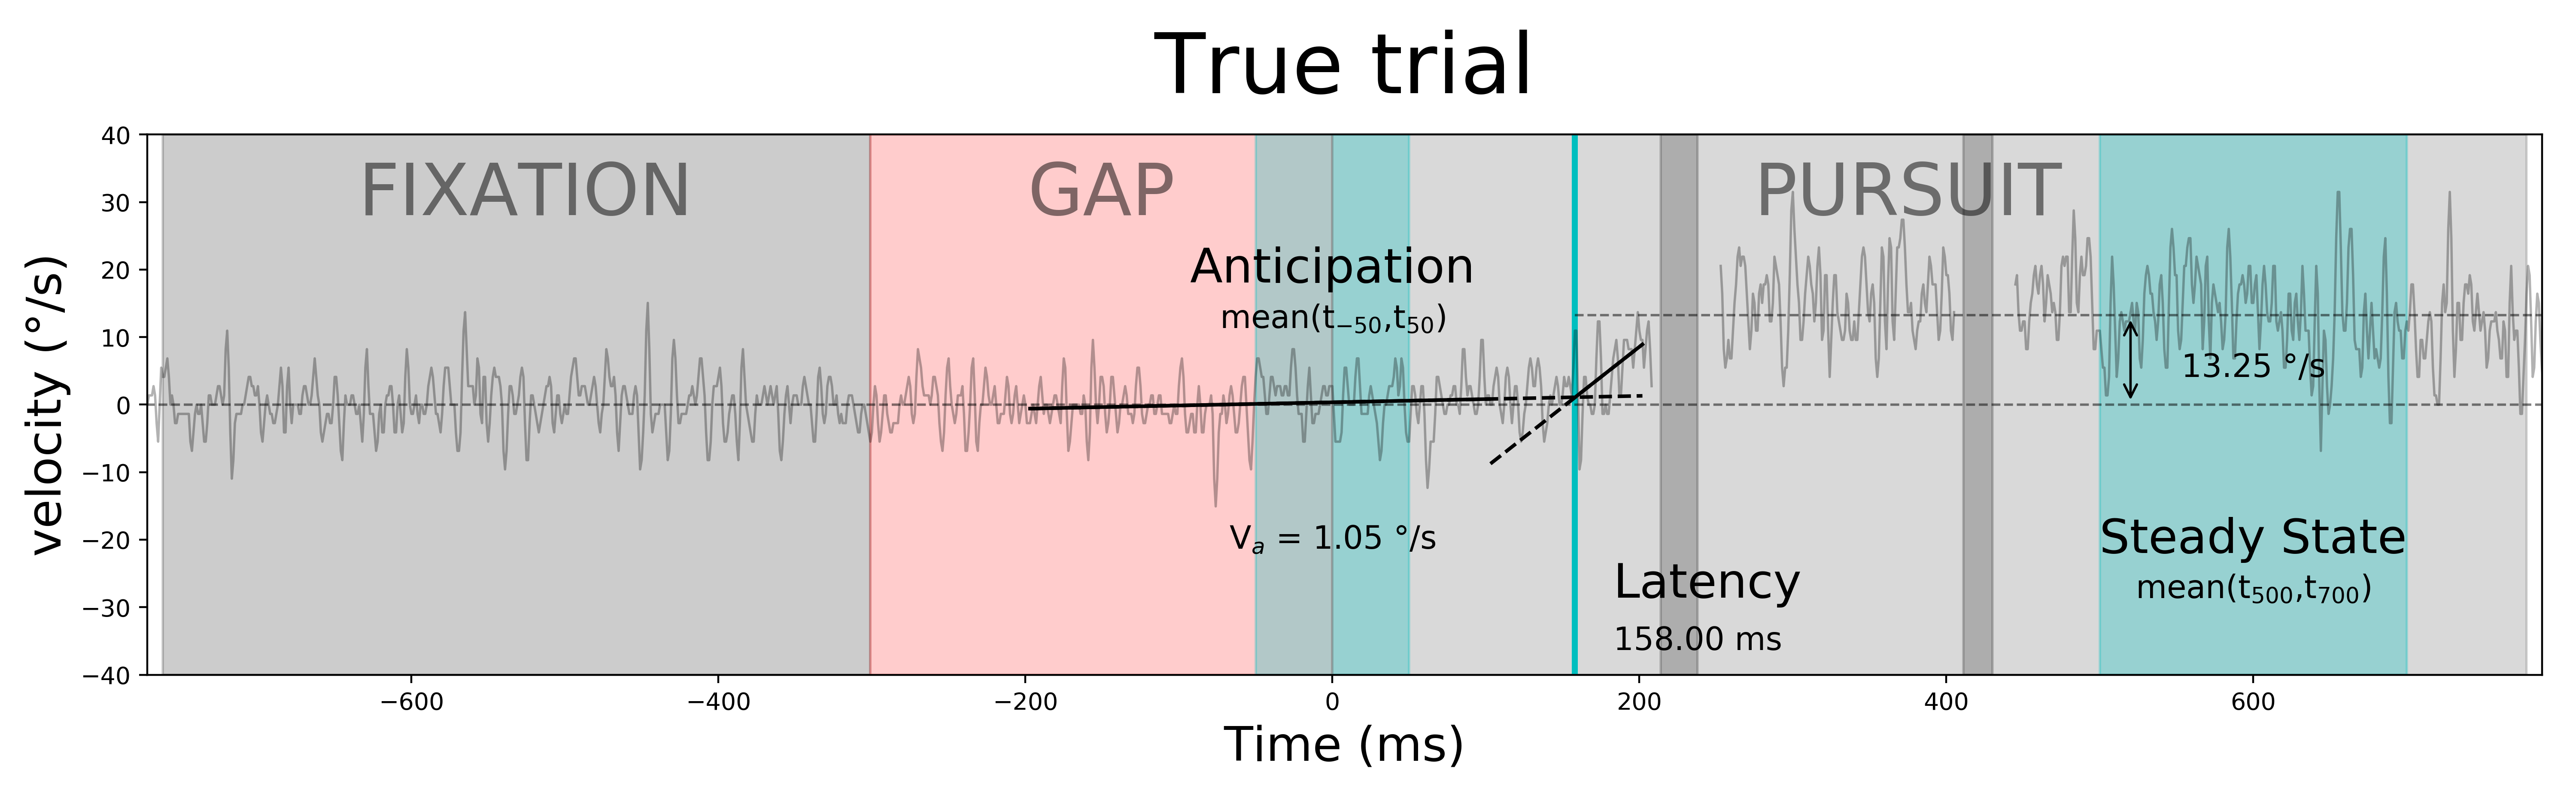
\includegraphics[width=0.455\columnwidth]{Old_methods_reel} %\includegraphics[width=0.313\columnwidth]
\vspace{\spacefig}
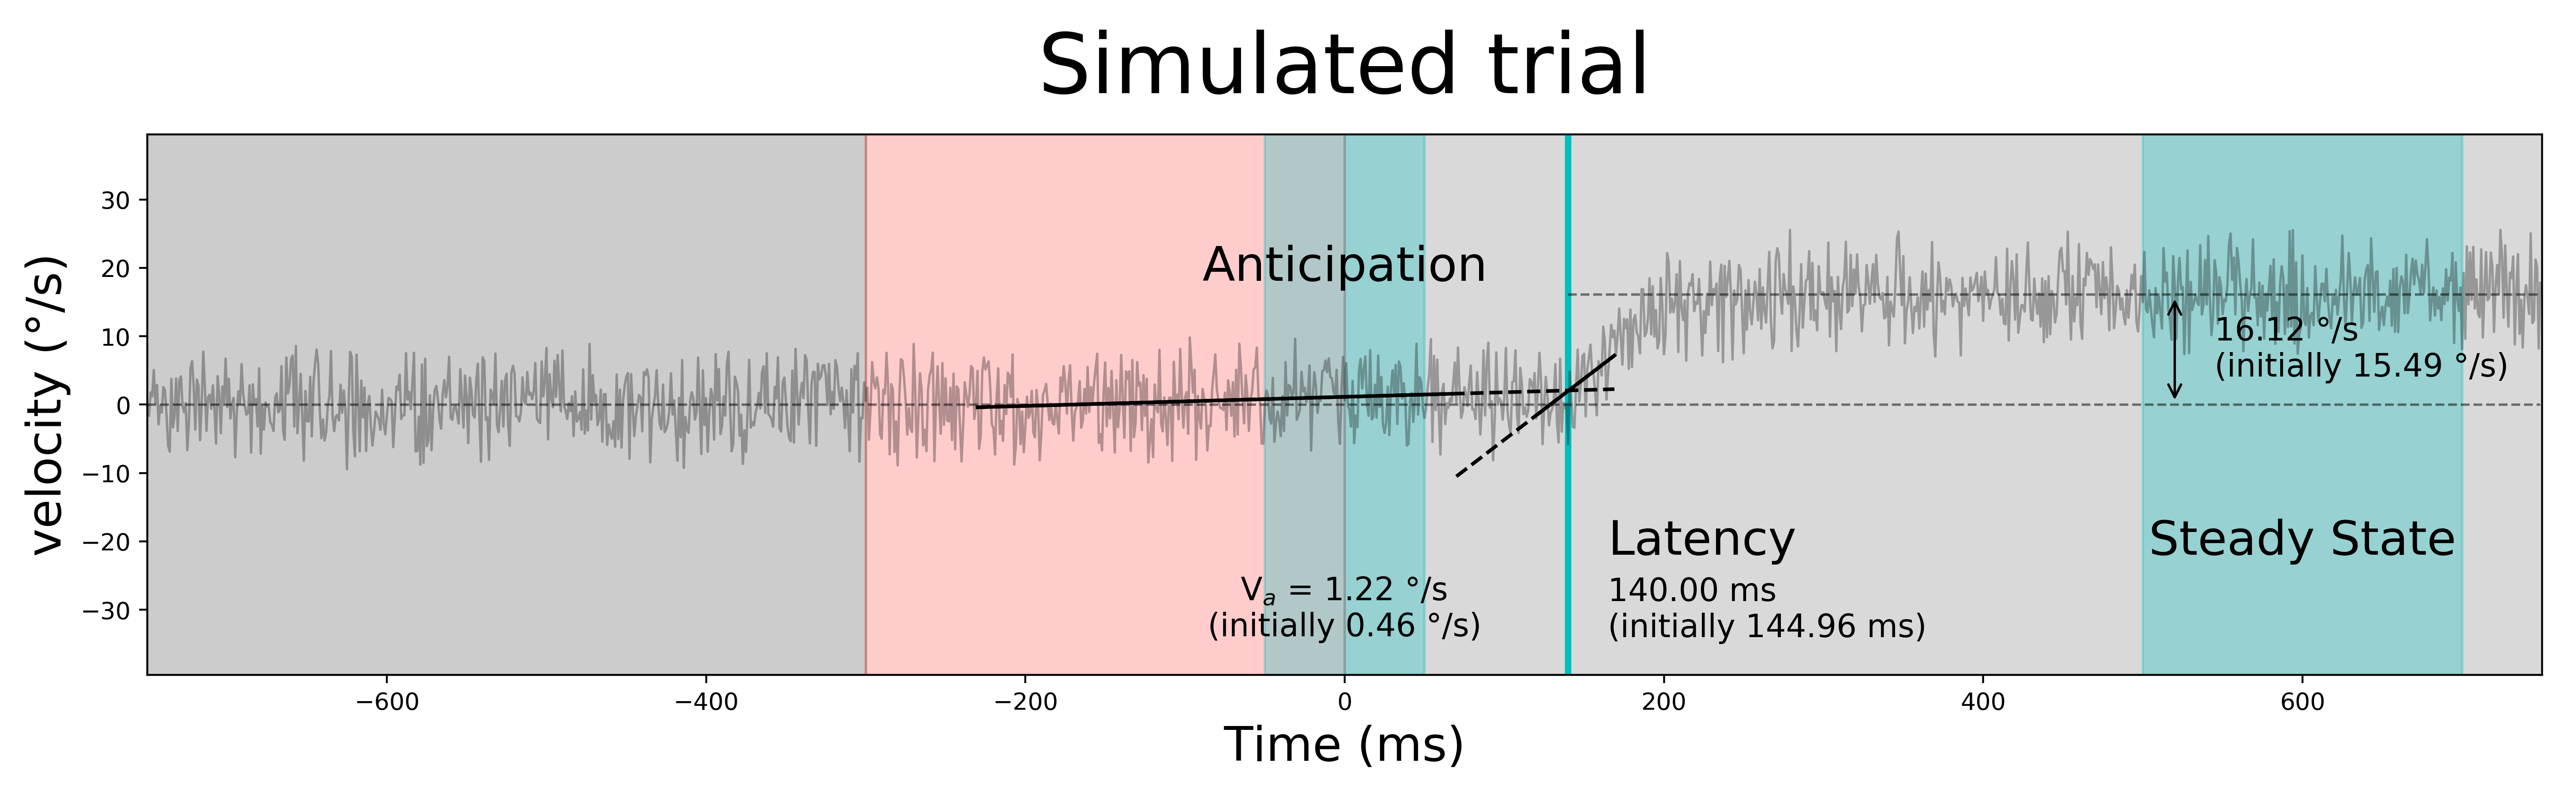
\includegraphics[width=0.455\columnwidth]{Old_methods_simulation}
 &&
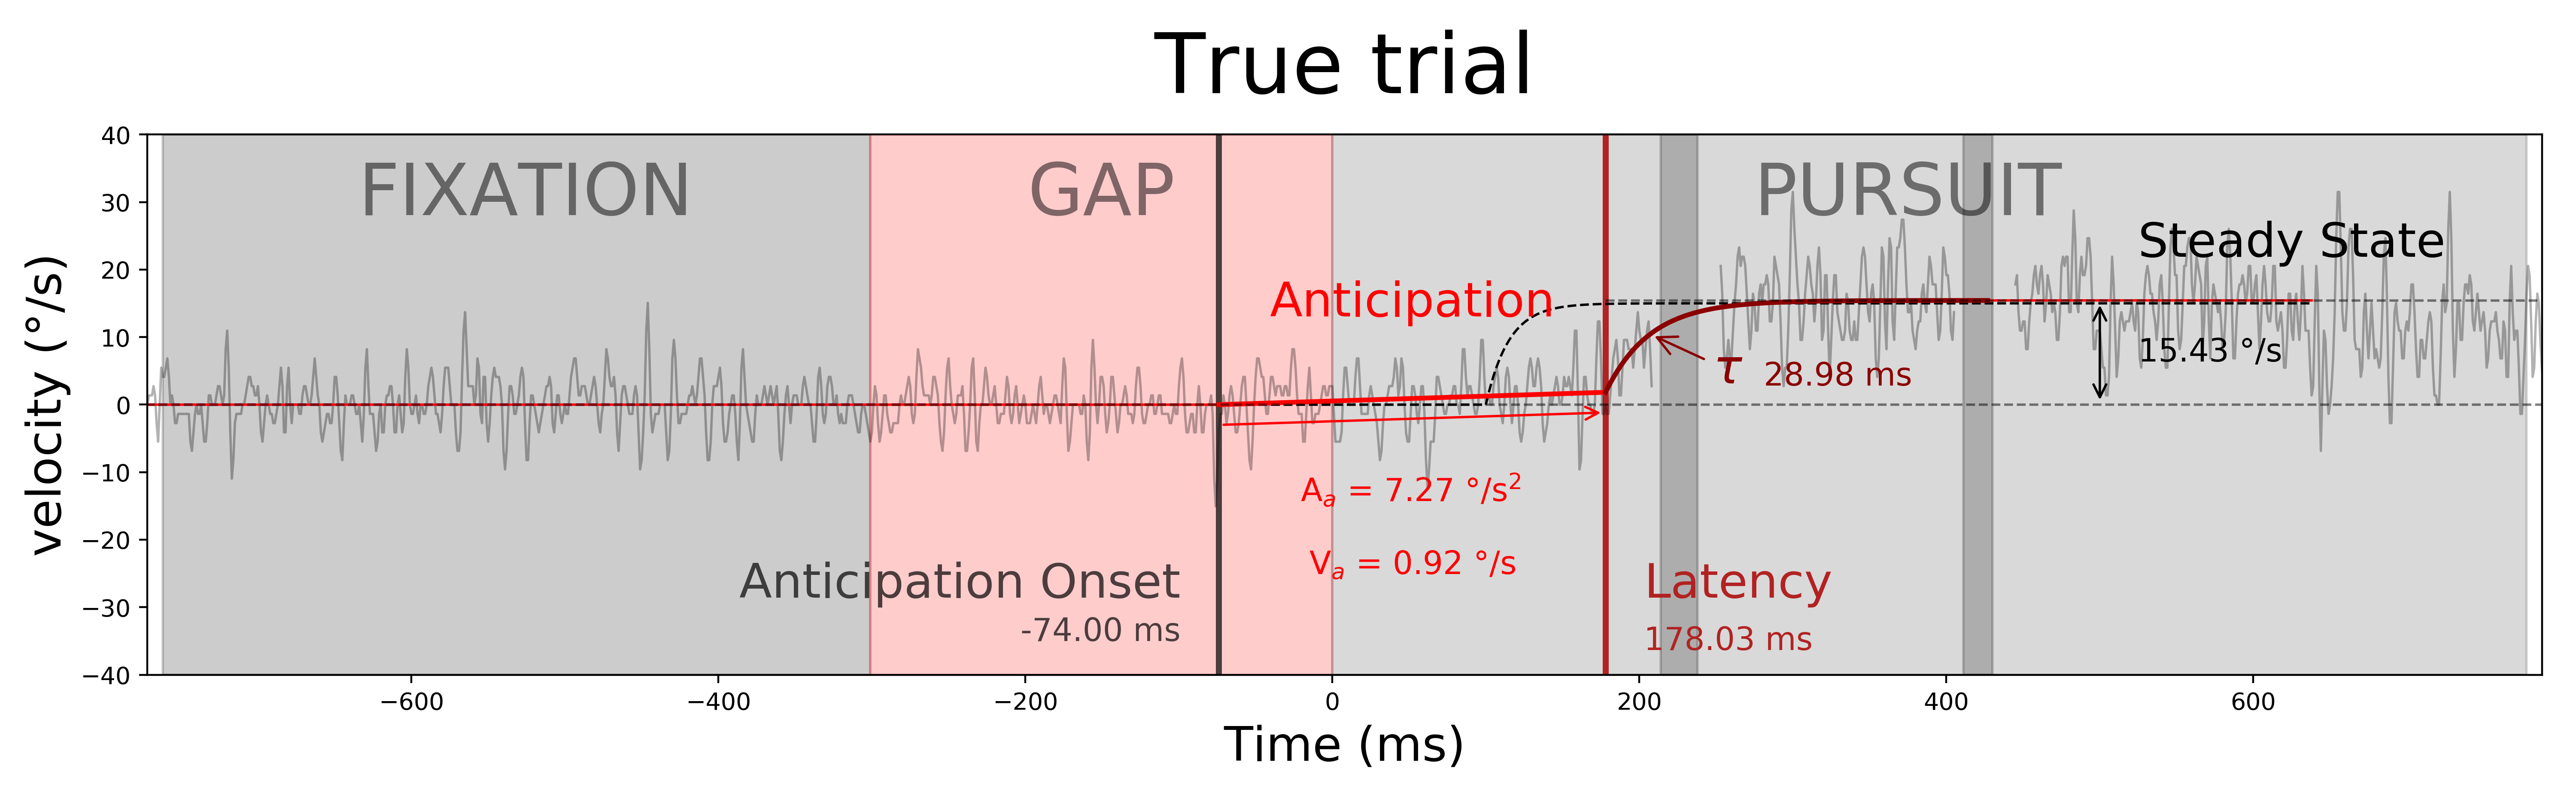
\includegraphics[width=0.455\columnwidth]{Fit_reel}
\vspace{\spacefig}
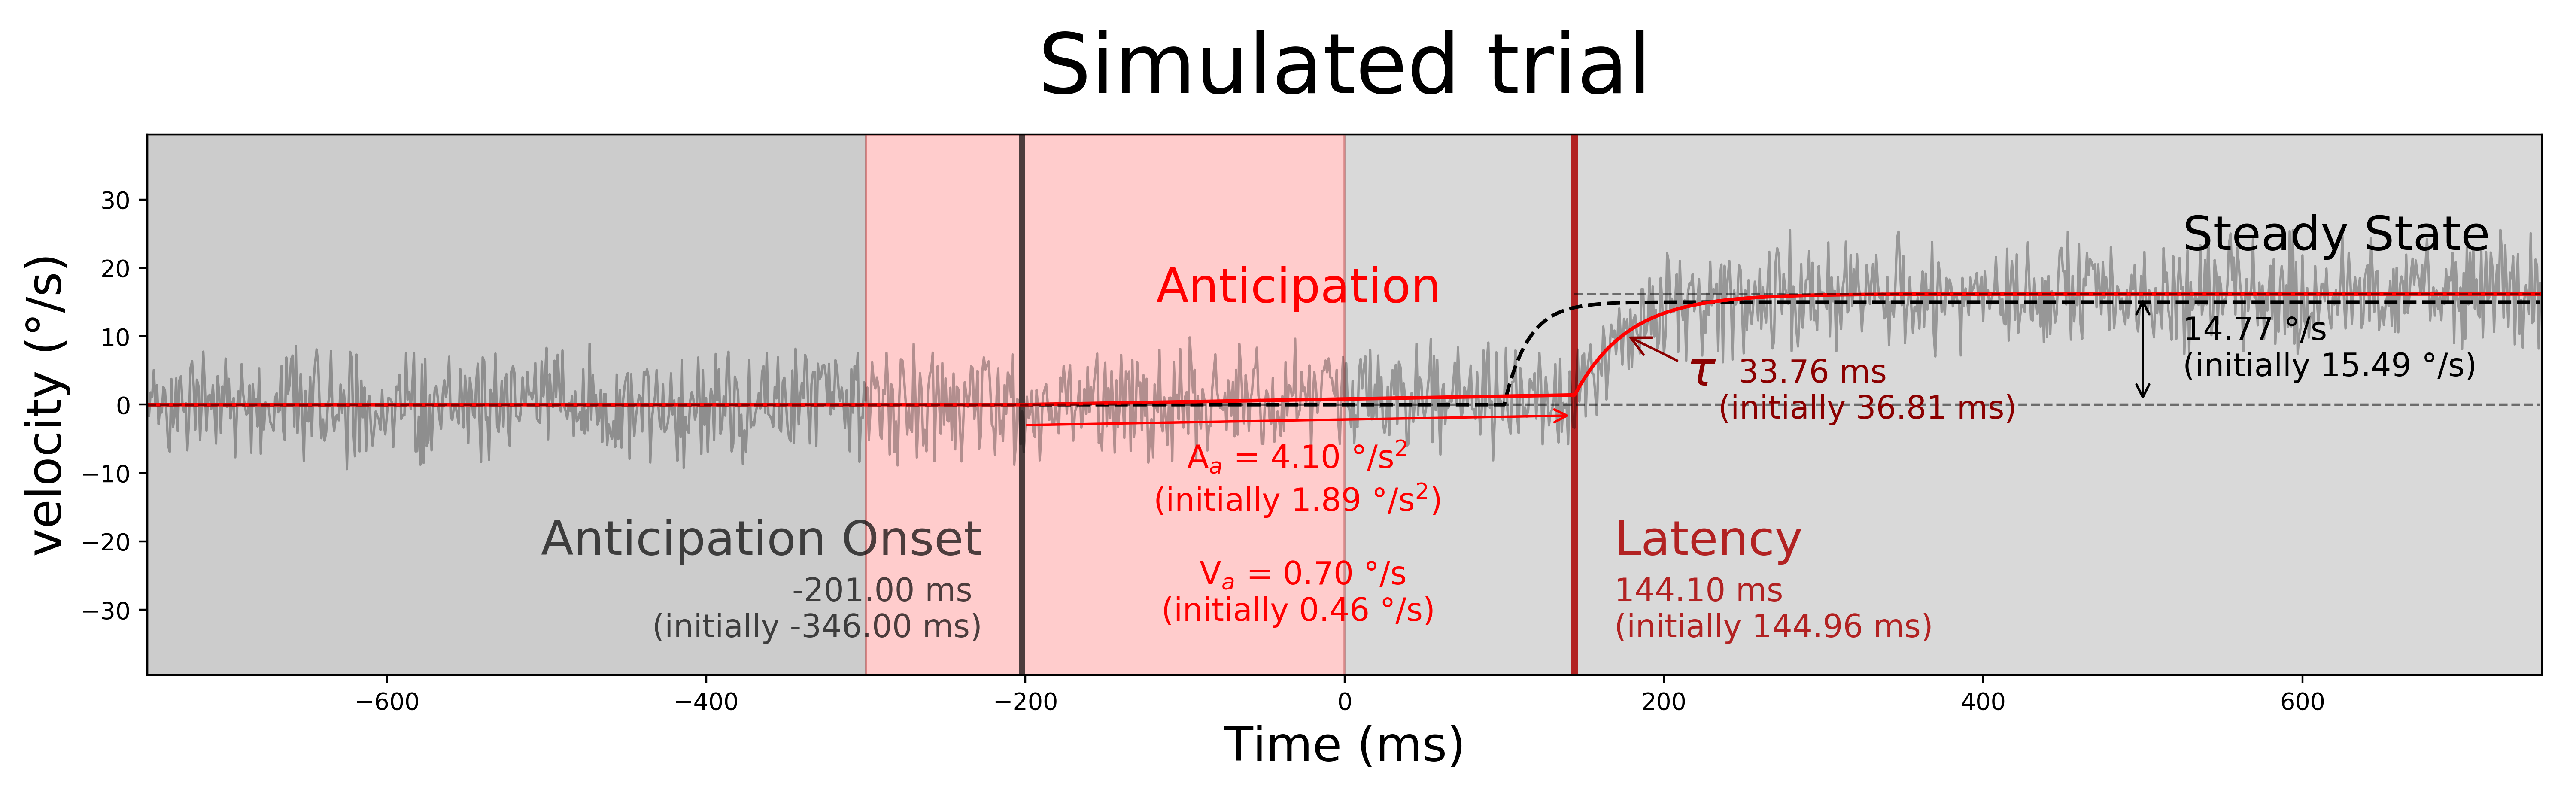
\includegraphics[width=0.455\columnwidth]{Fit_simulation}
\end{tabular}


\vspace{-.2\baselineskip} %\vspace{.5\baselineskip}

%----------------------------------------------------------------------------------------------------------
\section*{Results}
\vspace{-.8\baselineskip}

The true values are the values used to generate the original signal (S$_o$, noiseless simulated eye velocity) before adding random gaussian noise. %The true Anticipatory Velocity is the average S$_o$ from true Anticipation onset time to true Latency of visually-guided pursuit.
\vspace{-.7\baselineskip}
\begin{itemize}\setlength{\itemsep}{0ex}
\item The true Anticipatory Velocity (True V$_a$ 50 ( $^\circ/s$)) is the average S$_o$ from -50 to 50 ms.
\item The true Anticipatory Velocity (True V$_a$ onset ( $^\circ/s$)) is the average S$_o$ from true Anticipation onset time to true Latency of visually-guided pursuit.
\end{itemize}


\vspace{-0.7\baselineskip}
\begin{tabular}{p{0.313\columnwidth}m{0.03\columnwidth}p{0.313\columnwidth}m{0.03\columnwidth}p{0.313\columnwidth}}
\subsection*{Classical Methods}
&&
\subsection*{ANEMO Fitting Method}
&&
\end{tabular}

\vspace{-2\baselineskip}
\begin{tabular}{m{0.313\columnwidth}m{0.03\columnwidth}m{0.313\columnwidth}m{0.03\columnwidth}m{0.313\columnwidth}}
\includegraphics[width=0.293\columnwidth]{old_a_anti_true_classique_Full_2_\block}
\includegraphics[width=0.293\columnwidth]{old_latency_Full_\block}
\includegraphics[width=0.293\columnwidth]{old_max_Full_\block}
& &
\includegraphics[width=0.293\columnwidth]{old_a_anti_fit_true_Full_2_\block}
\includegraphics[width=0.293\columnwidth]{latency_Full_\block}
\includegraphics[width=0.293\columnwidth]{maxi_Full_\block}
& &
\includegraphics[width=0.293\columnwidth]{a_anti_Full_\block}
\includegraphics[width=0.293\columnwidth]{new_start_anti_Full_\block}
\includegraphics[width=0.293\columnwidth]{tau_Full_\block}
\end{tabular}


\vspace{.1\baselineskip}

%----------------------------------------------------------------------------------------------------------
%\begin{tabular}{p{0.485\columnwidth}m{0.03\columnwidth}p{0.485\columnwidth}}
\section*{Conclusions}
\vspace{-.8\baselineskip}
Compared with classical methods, the ANEMO fitting method proves more efficient for validating and categorizing tracking performance globally, including prediction-based anticipation.The optimisation of the code is still in progress. Moreover, this code is made available as an open-source package at \textbf{http://github.com/invibe/ANEMO}, allowing for the community to use and modify these methods.
%& &
{\tiny
\printbibliography
}

%\end{tabular}

%%%%%%%%%%%%%%%%%%%%%%%%%%%%%%%%
\end{document}%
